
\section*{Общая характеристика работы}

\newcommand{\actuality}{\underline{\textbf{\actualityTXT}}}
\newcommand{\progress}{\underline{\textbf{\progressTXT}}}
\newcommand{\aim}{\underline{{\textbf\aimTXT}}}
\newcommand{\tasks}{\underline{\textbf{\tasksTXT}}}
\newcommand{\novelty}{\underline{\textbf{\noveltyTXT}}}
\newcommand{\influence}{\underline{\textbf{\influenceTXT}}}
\newcommand{\methods}{\underline{\textbf{\methodsTXT}}}
\newcommand{\defpositions}{\underline{\textbf{\defpositionsTXT}}}
\newcommand{\reliability}{\underline{\textbf{\reliabilityTXT}}}
\newcommand{\probation}{\underline{\textbf{\probationTXT}}}
\newcommand{\contribution}{\underline{\textbf{\contributionTXT}}}
\newcommand{\publications}{\underline{\textbf{\publicationsTXT}}}


{\actuality} Открытые в  2007 году керровские оптические частотные гребенки в оптических микрорезонаторах \cite{DelHaye2007,Kippenberg2011} вызвали новую революцию в области метрологии. Керровские гребенки позволяют достичь уровня миниатюризации и энергоэффективности, труднодостижимого для гребенок, полученных с помощью фемтосекундных лазеров в режиме синхронизации мод, что в свою очередь позволяет существенно уменьшить размеры генераторов гребенок и создавать их на одном чипе, что в настоящее время исследуется во множестве лабораторий.

Основными преимуществами частотных гребенок из микрорезонаторов являются их компактность, высокая мощность, приходящаяся на каждую компоненту гребенки, и возможность получения частот повторения в диапазоне 10-1000 ГГц, важном для многих приложений, включая телекоммуникации высокой пропускной способности \cite{Pfeifle2014}, астрофизику \cite{Glenday2015}, синтез частот \cite{Ferdous2011}, радиофотонику и генерацию микроволн \cite{Xue2016,Savchenkov2008}. Оптическая частотная гребёнка может быть использована как высокостабильный калибровочный репер для прецизионной спектроскопии, как источник спектрально чистого СВЧ сигнала, а также для генерации фемтосекундных оптических импульсов – генераторы гребенки могут обеспечивать короткие периодические оптические импульсы с очень малым временным джиттером. Параметрический характер усиления обеспечивает широкополосность процесса в полосе, достигающей октавы. Подобный спектр гребенки может связывать оптический диапазон с микроволновым и наоборот. Кроме того, ширина полосы усиления ограничена только окном прозрачности материала микрорезонатора, что позволяет генерировать гребенки как в УФ, так и среднем ИК диапазонах.

В последние годы наблюдается быстрый и существенный прогресс в области керровских частотных гребенок. Гребенки были продемонстрированы в различных структурах, в том числе в кристаллических резонаторах из различных фторидов \cite{Savchenkov2008,Grudinin2012,Jost2015,Liang2011,DelHaye2011,Chembo2010,Grudinin2009}, в интегральных микрорезонаторах из нитрида кремния (SiN) \cite{Levy2010,Okawachi2011,Johnson2012,Huang2015}.

% {\progress}
% Этот раздел должен быть отдельным структурным элементом по
% ГОСТ, но он, как правило, включается в описание актуальности
% темы. Нужен он отдельным структурынм элемементом или нет ---
% смотрите другие диссертации вашего совета, скорее всего не нужен.

{\aim} данной работы является поиск методов генерации оптических частотных гребенок в микрорезонаторах при различной дисперсии групповой скорости на различных длинах волн накачки, экспериментальное получение солитонов в кристаллических микрорезонаторов и изучение их возможных приложений.

Для~достижения поставленной цели необходимо было решить следующие {\tasks}:
\begin{enumerate}
  \item Разработать численный метод моделирования динамики оптических частотных гребенок в микрорезонаторах.
  \item Разработать методику изготовления кристаллических микрорезонаторов с высокой добротностью.
  \item Создать экспериментальную установку для изучения кристаллических микрорезонаторов.
  \item Экспериментально получить солитонный режим генерации керровской гребенки, изучить его свойства и продемонстрировать практическое применение.
\end{enumerate}

{\novelty}
\begin{enumerate}
  \item На основе численного моделирования был предложен оригинальный метод генерации оптических частотных гребенок при нормальной дисперсии групповой скорости в резонаторе при отклонении дисперсионного закона.
  \item На основе численного моделирования был предложен оригинальный метод генерации оптических частотных гребенок при нормальной дисперсии групповой скорости в резонаторе при использовании двухчастотной или амлитудно-модулированной накачке.
  \item Впервые была продемонстрирована методика изготовления идентичных по форме кристаллических микрорезонаторов высокой добротности с различием по диаметру в 1 мкм.
  \item Впервые продемонстрирована возможность одновременнной генерации солитонов в идентичных микрорезонаторах, расположенных на одном кристаллическом цилиндре.
  \item Впервые продемонстрирована возможность одновременнной генерации солитонов в одном резонаторе на разных семействах пространственных мод распространяющихся как в одном, так и в противоположных направлениях. 
\end{enumerate}

{\influence} разработанной методики изготовления кристаллических микрорезонаторов заключается в возможности повторяемо изготавливать высокдобротные микрорезонаторы с заданными характеристиками. Экспериментальная демонстрация генерации двойных оптических в одном резонаторе на разных семействах мод имеет прямое приложение в устройствах спектроскопии поглощения и быстрого измерения расстояний. Экспериментальная демонстрация солитонного режима имеет прямое практическое применение как источника высокостабильного СВЧ сигнала на частоте повторения солитонов.

{\methods} В работе использовались как общенаучные методы: анализ, наблюдение, сравнение, эксперимент, так и специальные методы численного компьютерного моделирования.

{\defpositions}
\begin{enumerate}
  \item Первое положение
  \item Второе положение
  \item Третье положение
  \item Четвертое положение
\end{enumerate}

{\reliability} Достоверность полученных результатов определяется адекватностью использованных физических моделей и математических методов, выбранных для решения поставленных задач, корректностью использованных приближений, а также
соответствием результатов теоретических и численных расчетов и экспериментальных данных, и не вызывает сомнений. Результаты находятся в соответствии с результатами, полученными другими авторами.

Численная модель основана на решении системы нелинейных дифференциальных уравнений, полученных из уравнений Максвелла. Использовались широко известные численные методы решения ОДУ. В основе экспериментальных исследований лежали классические методы оптики и методики измерений физических величин.

{\probation}
Основные результаты работы докладывались~на:
\begin{enumerate}
  \item Microresonator Frequency Combs and Applications, Ascona, 2014
  \item CLEO/QELS, San Jose, 2014
  \item PQE-2015, Snowbird UT, 2015
  \item CLEO, San Jose, 2015
  \item XV Всероссийская школа-семинар "Физика и применение микроволн" имени профессора А.П. Сухорукова ( "Волны-2015", Красновидово, 2015
  \item Third International Conference on Quantum Technologies (ICQT 2015), Москва, 2015
  \item Photonics West, Сан-Франциско, 2016
  \item EMN Optical Communications Meeting, Дубай, 2016
  \item SPIE Photonics West, Сан-Франциско, 2016
  \item Progress In Electromagnetics Research Symposium (PIERS 2017 in St Petersburg), Санкт-Петербург, 2017
  \item XVI Всероссийская школа-семинар "Физика и применение микроволн" имени профессора А.П. Сухорукова ( "Волны-2017"), Красновидово, 2017
  \item CLEO Europe & EQEC 2017
\end{enumerate}


{\contribution} Все результаты, вошедшие в диссертационную работу, получены либо лично
автором, либо совместно с соавторами работ, опубликованных по теме диссертации.

%\publications\ Основные результаты по теме диссертации изложены в ХХ печатных изданиях~\cite{Sokolov,Gaidaenko,Lermontov,Management},
%Х из которых изданы в журналах, рекомендованных ВАК~\cite{Sokolov,Gaidaenko},
%ХХ --- в тезисах докладов~\cite{Lermontov,Management}.

\ifnumequal{\value{bibliosel}}{0}{% Встроенная реализация с загрузкой файла через движок bibtex8
    \publications\ Основные результаты по теме диссертации изложены в 16 печатных изданиях,
    7 из которых изданы в журналах, рекомендованных ВАК,
    9 "--- в тезисах докладов.%
}{% Реализация пакетом biblatex через движок biber
%Сделана отдельная секция, чтобы не отображались в списке цитированных материалов
    \begin{refsection}[vak,papers,conf]% Подсчет и нумерация авторских работ. Засчитываются только те, которые были прописаны внутри \nocite{}.
        %Чтобы сменить порядок разделов в сгрупированном списке литературы необходимо перетасовать следующие три строчки, а также команды в разделе \newcommand*{\insertbiblioauthorgrouped} в файле biblio/biblatex.tex
        \printbibliography[heading=countauthorvak, env=countauthorvak, keyword=biblioauthorvak, section=1]%
        \printbibliography[heading=countauthorconf, env=countauthorconf, keyword=biblioauthorconf, section=1]%
        \printbibliography[heading=countauthornotvak, env=countauthornotvak, keyword=biblioauthornotvak, section=1]%
        \printbibliography[heading=countauthor, env=countauthor, keyword=biblioauthor, section=1]%
        \nocite{%Порядок перечисления в этом блоке определяет порядок вывода в списке публикаций автора
                vakbib1,vakbib2,%
                confbib1,confbib2,%
                bib1,bib2,%
        }%
        \publications\ Основные результаты по теме диссертации изложены в~\arabic{citeauthor}~печатных изданиях,
        \arabic{citeauthorvak} из которых изданы в журналах, рекомендованных ВАК,
        \arabic{
        authorconf} "--- в~тезисах докладов.
    \end{refsection}
    \begin{refsection}[vak,papers,conf]%Блок, позволяющий отобрать из всех работ автора наиболее значимые, и только их вывести в автореферате, но считать в блоке выше общее число работ
        \printbibliography[heading=countauthorvak, env=countauthorvak, keyword=biblioauthorvak, section=2]%
        \printbibliography[heading=countauthornotvak, env=countauthornotvak, keyword=biblioauthornotvak, section=2]%
        \printbibliography[heading=countauthorconf, env=countauthorconf, keyword=biblioauthorconf, section=2]%
        \printbibliography[heading=countauthor, env=countauthor, keyword=biblioauthor, section=2]%
        \nocite{vakbib2}%vak
        \nocite{bib1}%notvak
        \nocite{confbib1}%conf
    \end{refsection}
}
%При использовании пакета \verb!biblatex! для автоматического подсчёта
%количества публикаций автора по теме диссертации, необходимо
%их~здесь перечислить с использованием команды \verb!\nocite!.
 % Характеристика работы по структуре во введении и в автореферате не отличается (ГОСТ Р 7.0.11, пункты 5.3.1 и 9.2.1), потому её загружаем из одного и того же внешнего файла, предварительно задав форму выделения некоторым параметрам

%Диссертационная работа была выполнена при поддержке грантов ...

%\underline{\textbf{Объем и структура работы.}} Диссертация состоит из~введения, четырех глав, заключения и~приложения. Полный объем диссертации \textbf{ХХХ}~страниц текста с~\textbf{ХХ}~рисунками и~5~таблицами. Список литературы содержит \textbf{ХХX}~наименование.

%\newpage
\section*{Содержание работы}
Во \underline{\textbf{введении}} обосновывается актуальность
исследований, проводимых в~рамках данной диссертационной работы,
приводится обзор научной литературы по изучаемой проблеме,
формулируется цель, ставятся задачи работы, излагается научная новизна
и практическая значимость представляемой работы.


\underline{\textbf{Первая глава}} посвящена обзору литературы, посвященной генерации оптических частотных гребенок и солитонов в микрорезонаторах. Над развитием этой новой области работают около 10 экспериментальных групп и еще несколько теоретических групп. За 11 прошедших с открытия лет был проведен обширный теоретический анализ и численное моделирование богатой нелинейной динамики процесса формирования оптических гребенок, были проведены эксперименты, демонстрирующие их фундаментальные свойства и важнейшие практически применения. Дан обзор многочисленных работ посвященных теоретическому и численному моделированию динамики генерации оптических гребенок, как шумных, так и высококогерентных. Рассмотрены работы посвященные экспериментальной демонстрации оптических гребенок и солитонов в кристаллических, интегральных резонаторах из различных материалов при накачке на длинах волн от ближнего ИК до среднего ИК. Сделан обзор экспериментальных демонстраций различных эффектов: излучения дисперсионных волн, Рамановского сдвига центра солитона, бризерных режимов солитонов, Стоксовы солитоны, различных методов контроля дисперсии групповой скорости резонаторов.

Наблюдение диссипативных керровских солитонов в микрорезонаторах вызвало не только интерес к изучению богатой нелинейной физики солитонов, но и демонстрации множества применений в высокоточной метрологии и других технологиях. Даны обзоры продемонстрированных применений оптических частотных гребенок и солитонов: оптические часы, перенос точности СВЧ стандарта частоты в оптический диапазон, калибровка астрономических эшелле-спектрографов, прямая спектроскопия поглощения веществ с использованием двух оптических гребенок, в роли оптического источника в установке для спектрального уплотнения телекоммуникационных каналов и когерентной передачи данных, в роли источника СВЧ сигнала с низким уровнем фазового шума, в роли источника импульсов для быстрого измерения расстояний (ЛИДАР), или как интегральный синтезатор оптических частот.

\underline{\textbf{Вторая глава}} посвящена численному моделированию динамики генерации оптических частотных гребенок и солитонов исследованию возможных режимов и поиску оптимальных параметров.

В п. 2.1 представлен вывод системы уравнений для связанных мод из уравнений Максвелла в оптически нелинейном микрорезонаторе. Показана эквивалентность этой модели и уравнения Луджиато-Лефевера. Это уравнение получается из нелинейного уравнения Шредингера (НУШ) добавлением слагаемых, отвечающих за диссипацию и накачку. НУШ является интегрируемой системой, для поиска решений которой используется метод обратной задачи рассеяния. Уравнение Луджиато-Лефевера не является интегрируемой системой, необходимо численное моделирование.

В п. 2.2 описаны используемые численные методы с их сравнением: метод Рунге-Кутты с адаптивным шагом и оптимизацией для быстрого вычисления нелинейной суммы, а также Фурье метод расщепления по параметрам для численного решения уравнения Луджиато-Лефевера. Был реализован удобный программный интерфейс в среде Matlab для моделирования обоими методами при различной настройке всех параметров.

В п. 2.3 по результатам моделирования были выявлены параметры и режимы, при которых возможно достижение солитонного режима (рис. \ref{100modes}). Был учтен нагрев резонатора, различная связь и мощность накачки, а также ключевой параметр - отстройка частоты лазера накачки от собственной частоты моды резонатора ($\zeta_0$). Именно найденный при численном моделировании метод сканирования частоты лазера накачки, позволил экспериментально обнаружить солитоны в микрорезонаторах. Было проведено моделирование при различных дисперсионных законах, численно получена генерация дисперсионной волны (оптического аналога Черенковского излучения), мощность и положение спектрального пика при этом хорошо совпала с экспериментальными значениями. Выявлены диапазоны параметров дисперсии высоких порядков, препятствующие образованию солитонов, а также влияние эффекта нормального расщепления мод вблизи моды накачки на возможность генерации солитонов. Результаты моделирования хорошо совпали с экспериментальными данными из литературы.

\begin{figure}
  \centering
%  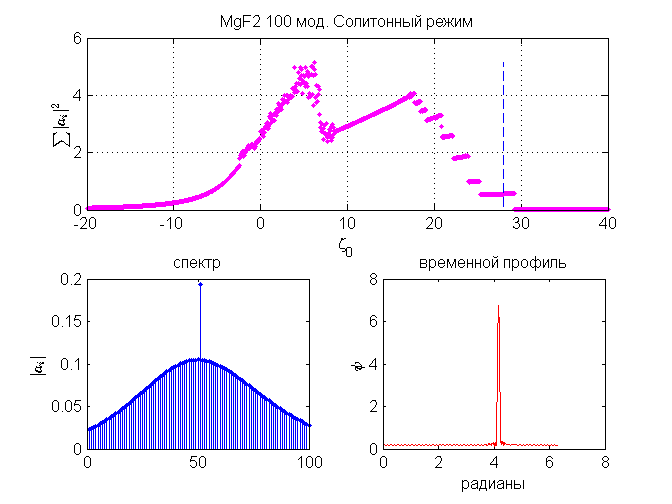
\includegraphics[width = 1\textwidth,height=0.5\textheight]{mgf2_100modes}
 % 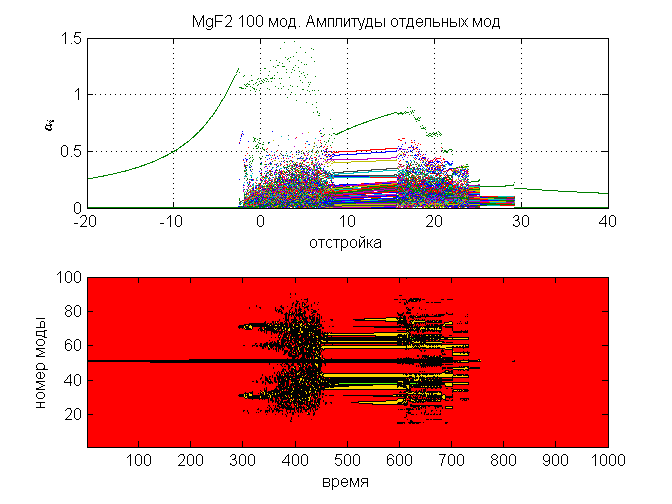
\includegraphics[width = 1\textwidth,height=0.5\textheight]{mgf2_100modes_modal}
  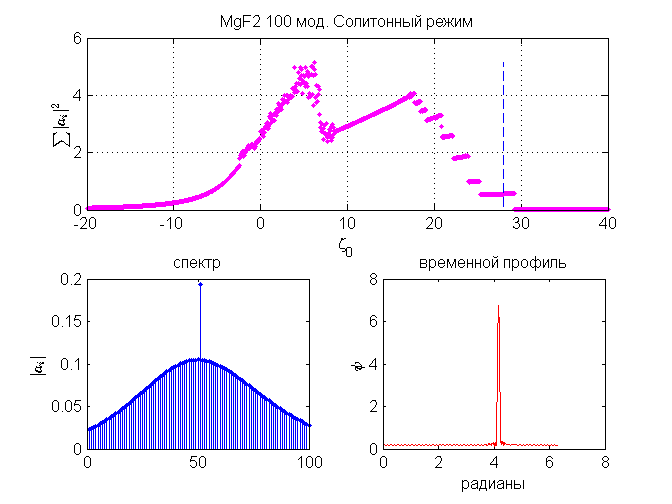
\includegraphics[width = 0.5\textwidth]{mgf2_100modes}
  \caption{Моделирование динамики генерации оптической частотной гребенки для 100 мод в резонаторе из $MgF_2$. Мощность накачки $100$ мВт. Лазер накачки перестраивается по частоте линейно во времени. На верхнем графике суммарного поля внутри резонатора видны характерные ступеньки, соответствующие солитонному режиму. В нижнем ряду показан спектр и соответствующий ему временной профиль солитона на указанной пунктиром отстройке $\zeta_0$.}
  \label{100modes}
\end{figure}

В п. 2.4 и 2.5 с помощью численного моделирование динамики оптических гребенок в микрорезонаторах с нормальной дисперсией групповой, было найдено два новых метода генерации темных солитоноподобных локализованных структур (рис. \ref{platicons}): 1) локальное изменение дисперсионного закона вблизи моды накачки; 2) использование двухчастотной или амплитудно-модулированной накачки с частотой модуляции строго равной области свободной дисперсии микрорезонатора. В обоих случаях были исследованы области существования и мягкого возбуждения оптических гребенок из вакуумных флуктуаций в модах резонатора, определены зависимости от величины дисперсии, мощности накачки, глубины модуляции или величины сдвига моды накачки по частоте. Показано значительное увеличение мощности оптической гребенки в режиме нормальной дисперсии. Предложенный метод был позже реализован экспериментально в других группах.

\begin{figure}
  \centering
  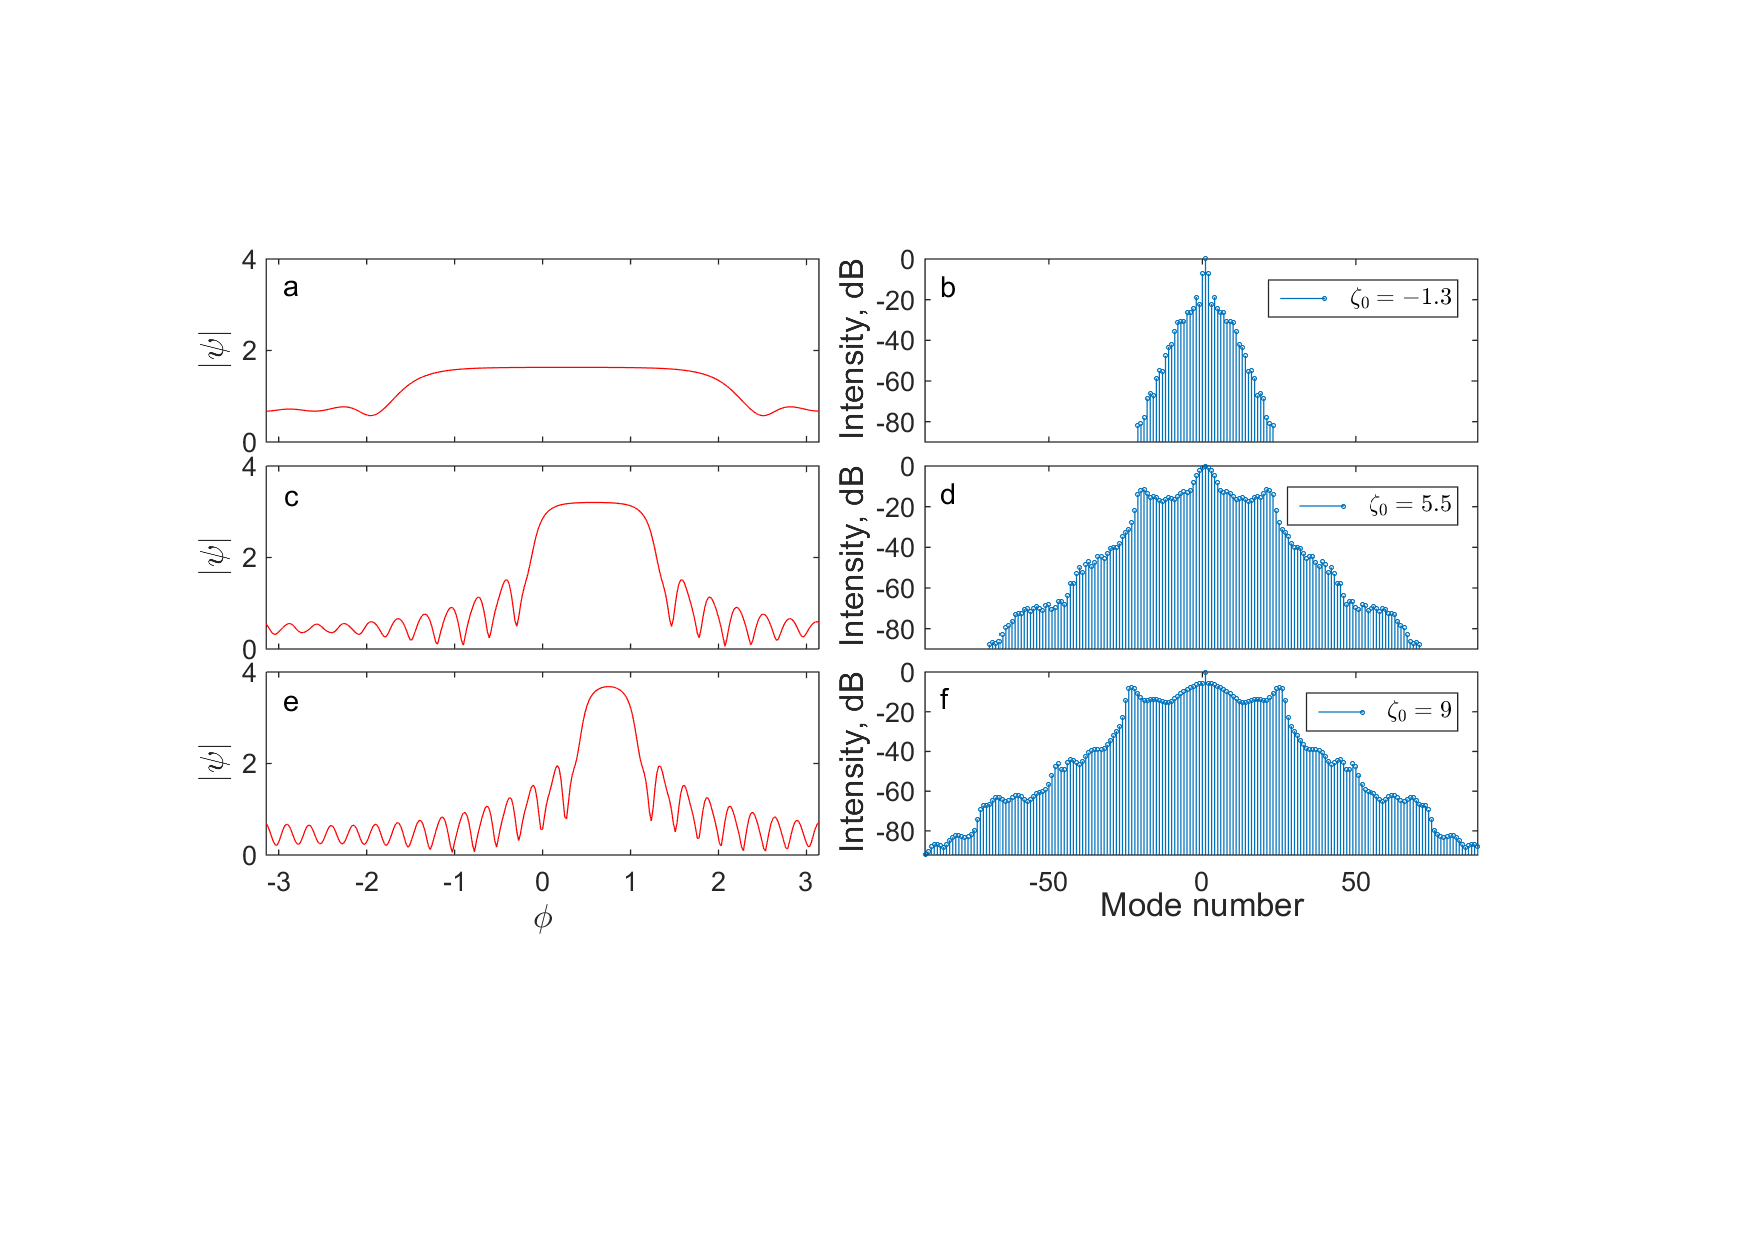
\includegraphics[width = 0.7\textwidth,height=0.4\textheight]{platicons}
  \caption{Характерные временные профили поля (зависимость суммарного поля $\Psi$ от азимутальной координаты $\pshi$) внутри резонатора с нормальной дисперсией групповой скорости (левая панель) и спектры темных солитоноподобных локализованных структур для различных значений отстройки частоты лазера (правая панель), получающиеся при локальном изменении дисперсионного закона вблизи моды накачки.}
  \label{platicons}
\end{figure}

Результаты главы 2 были опубликованы в статьях с номерами 1,2,3,5 из списка публикаций.

\underline{\textbf{Третья глава}} посвящена экспериментальному исследованию методов генерации оптических частотных гребенок и солитонов в кристаллических микрорезонаторах и изучению их свойств.

В п. 3.1 разработана методика изготовления кристаллических микрорезонаторов методом алмазного точения с последующей полировкой алмазными суспензиями. Даны практические замечания по воспроизводимому изготовлению кристаллических микрорезонаторов заданной геометрии и высокой добротности. В ходе работы были изготовлены резонаторы с добротностью не менее $10^8$ из кристаллических материалов $MgF_2,BaF_2,CaF_2,LiNbO_3,LiF,YLiF:Yb$ и с меньшей добротностью из других материалов: $LiTaO_3,SiO_2,TGG,YLiF:Tm$. Методика позволяет воспроизводимо изготавливать микрорезонаторы с заданной геометрией с точность до 1 мкм. Минимальный диаметр изготовленных резонаторов составил 100 мкм, максимальный 16 мм. Были успешно изготовлены резонаторы с микровыступами, оптическое поле было локализовано в прямоугольном выступе на образующей цилиндра размером 5 на 10 мкм (см. рис. \ref{cavity_polished}).

\begin{figure}[ht]
  \begin{minipage}[ht]{0.32\linewidth}\centering
    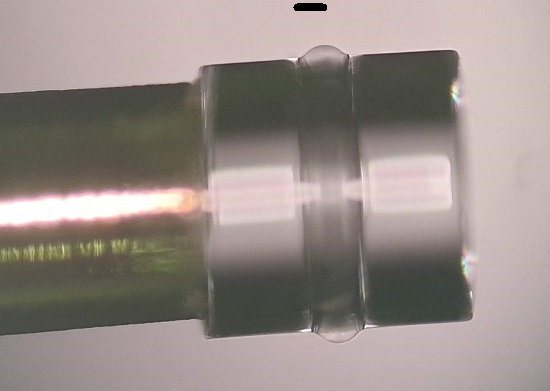
\includegraphics[width=1\linewidth]{caity1mm_polished}
  \end{minipage}
  \hfill
  \begin{minipage}[ht]{0.32\linewidth}\centering
    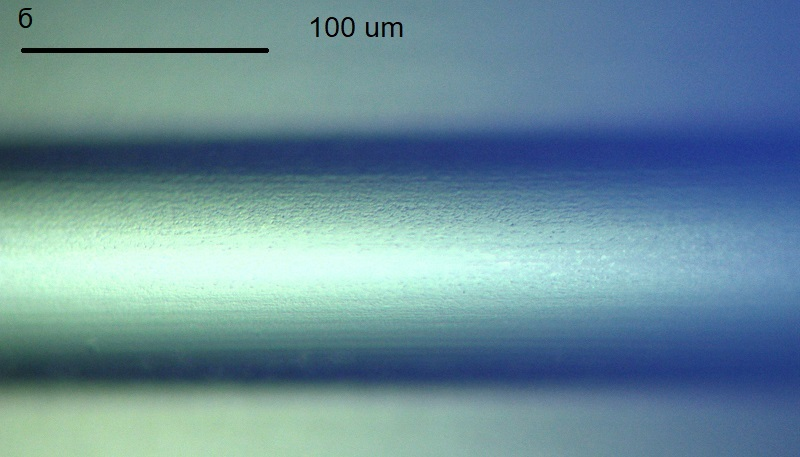
\includegraphics[width=1\linewidth]{protrusion_unpolished}
  \end{minipage}
  \hfill
  \begin{minipage}[ht]{0.32\linewidth}\centering
    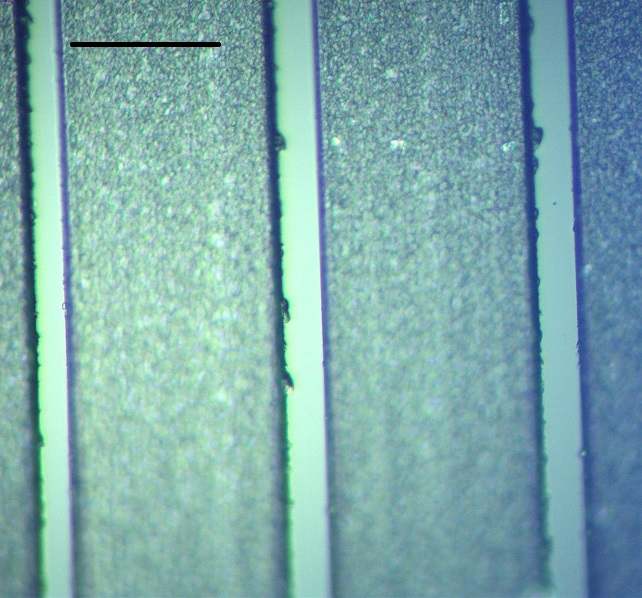
\includegraphics[width=1\linewidth]{protrsuion_rect}
  \end{minipage}
  \caption{Слева фото отполированного резонатора диаметром 1 мм на латунной подставке. По центру фото поверхности резонатора из $MgF_2$ сразу после точения, в котором достигается добротность $10^6$. Справа фрагмент поверхности резонатора с прямоугольными выступами размером 5 на 20, 25 мкм. Масштаб 100 мкм дан черным отрезком.}
  \label{cavity_polished}
\end{figure}


Дано описание экспериментальной установки, использующейся в большинстве экспериментов. Экспериментально продемонстрирована генерация шумных оптических частотных в резонаторах из $MgF_2,BaF_2$ и солитонного режима в $MgF_2$/ Измерены термооптические мод в резонаторе из $BaF_2$, в этом же материале наблюдались эффекты вынужденного комбинационного рассеяния и вынужденного рассеяния Мандельштама-Бриллюэна при накачке на длине волны 1550 нм, определены из частоты и ширины соответствующих сигналов биений.

Продемонстрирован солитонный режим генерации гребенки, показан метод достижения односолитонного режима с помощью амплитудной модуляции накачки на частоте повторения солитона. Также этим же методом показана стабилизация частоты повторения солитона из-за эффекта затягивания со значительным улучшением стабильности на больших временах.

%Можно сослаться на свои работы в автореферате. Для этого в файле
%\verb!Synopsis/setup.tex! необходимо присвоить положительное значение
%счётчику \verb!\setcounter{usefootcite}{1}!. В таком случае ссылки на
%работы других авторов будут подстрочными.
%\ifnumgreater{\value{usefootcite}}{0}{
%Изложенные в третьей главе результаты опубликованы в~\cite{vakbib1, vakbib2}.
%}{}
%Использование подстрочных ссылок внутри таблиц может вызывать проблемы.

В \underline{\textbf{четвертой главе}} приведены методы генерации двойных оптических гребенок и солитонов в кристаллических микрорезонаторах.

Экспериментально показана генерация двух солитонных оптических гребенок в двух резонаторах на одном цилиндре.

Экспериментально продемонстрирована генерация солитонных оптических гребенок в одном резонаторе на разных семействах мод в одном направлении.

Экспериментально продемонстрирована генерация солитонных оптических гребенок в одном резонаторе на разных семействах мод в противоположных направлениях. Продемонстрировано применение метода для прямой спектроскопии поглощения веществ.

Экспериментально продемонстрирована генерация солитонных оптических гребенок в одном резонаторе на одном семействе мод в противоположных направлениях

В \underline{\textbf{заключении}} приведены основные результаты работы, которые заключаются в следующем:
%% Согласно ГОСТ Р 7.0.11-2011:
%% 5.3.3 В заключении диссертации излагают итоги выполненного исследования, рекомендации, перспективы дальнейшей разработки темы.
%% 9.2.3 В заключении автореферата диссертации излагают итоги данного исследования, рекомендации и перспективы дальнейшей разработки темы.
\begin{enumerate}
  \item Численные исследования модели уравнений связанных мод показали, что в высокодобротных микрорезонаторах возможна генерация оптических временных солитонов, были изучены диапазоны параметров и условия, влияющие на их эффективную генерацию.
  \item Математическое моделирование показало, что при нормальной ДГС резонатора возможна генерация темных солитоноподобных структур при условии наличия изменения в законе дисперсии или при использовании двухчастотной или амплитудно-модулированной накачки. 
  \item Для выполнения экспериментальных исследований была разработана методика изготовления кристаллических микрорезонаторов методом алмазного точения и полировки алмазными суспензиями.
  \item Экспериментально была продемонстрирована генерация оптических солитонов в резонаторах из $MgF_2$ с ОСД от $8.5$ до $27$ ГГц. При активной стабилизации температуры и отстройки частоты лазера накачки солитон существовал длительное время, достаточное для экспериментальной демонстрации применений.
  \item Впервые продемонстрирована возможность одновременнной генерации солитонов в идентичных микрорезонаторах, расположенных на одном кристаллическом цилиндре.
  \item Впервые продемонстрирована возможность одновременнной генерации солитонов в одном резонаторе на разных семействах пространственных мод, распространяющихся как в одном, так и в противоположных направлениях.
  \item Для дальнейших исследований в данной области важной задачей является экспериментальная демонстрация широких, октавных гребенок в солитонном режиме, гребенок в кристаллических резонаторах с нормальной дисперсией. Из новых практических применений возможна демонстрация фотонного АЦП с использованием двойных оптических гребенок, демонстрация калибровки астрономических эшелле спектрометров.
\end{enumerate}



%\newpage
%При использовании пакета \verb!biblatex! список публикаций автора по теме
%диссертации формируется в разделе <<\publications>>\ файла
%\verb!../common/characteristic.tex!  при помощи команды \verb!\nocite!

\ifdefmacro{\microtypesetup}{\microtypesetup{protrusion=false}}{} % не рекомендуется применять пакет микротипографики к автоматически генерируемому списку литературы
\ifnumequal{\value{bibliosel}}{0}{% Встроенная реализация с загрузкой файла через движок bibtex8
  %\renewcommand{\bibname}{\large \authorbibtitle}
  %\nocite{*}
  %\insertbiblioauthor           % Подключаем Bib-базы
  \insertbibliofull
  %\insertbiblioother   % !!! bibtex не умеет работать с несколькими библиографиями !!!
}{% Реализация пакетом biblatex через движок biber
  \ifnumgreater{\value{usefootcite}}{0}{
%  \nocite{*} % Невидимая цитата всех работ, позволит вывести все работы автора
  \insertbiblioauthorcited      % Вывод процитированных в автореферате работ автора
  }{
  \insertbiblioauthor           % Вывод всех работ автора
%  \insertbiblioauthorgrouped    % Вывод всех работ автора, сгруппированных по источникам
%  \insertbiblioauthorimportant  % Вывод наиболее значимых работ автора (определяется в файле characteristic во второй section)
  \insertbiblioother            % Вывод списка литературы, на которую ссылались в тексте автореферата
  }
}
\ifdefmacro{\microtypesetup}{\microtypesetup{protrusion=true}}{}

